\documentclass[aspectratio=169]{beamer}
\usepackage{color,amsmath}
\usepackage{subfigure}
\usepackage{booktabs}
\usepackage{framed}
\usepackage{comment}

\def\vf{\vfill}

%%%%%%%%%%%%%%%%%%%%%%%%%%
\title[]{Preview of Lab\\(03-07)}
\author[]{Matthew J. Salganik\\Department of Sociology\\Princeton University}
\date[]{Soc 596: Computational Social Science\\Fall 2016
\vfill
\begin{flushright}
\vspace{0.6in}

\includegraphics[width=0.1\textwidth]{figures/cc.png}
\end{flushright}
}
\begin{document}
%%%%%%%%%%%%%%%%%%%%%%%%%%
\frame{\titlepage}
%%%%%%%%%%%%%%%%%%%%%%%%%%
\begin{frame}

\begin{center}

\includegraphics[width=0.7\textwidth]{figures/goel_non-representative_2016_title}
\end{center}

\end{frame}
%%%%%%%%%%%%%%%%%%%%%%%%%%%
\begin{frame}

\begin{center}
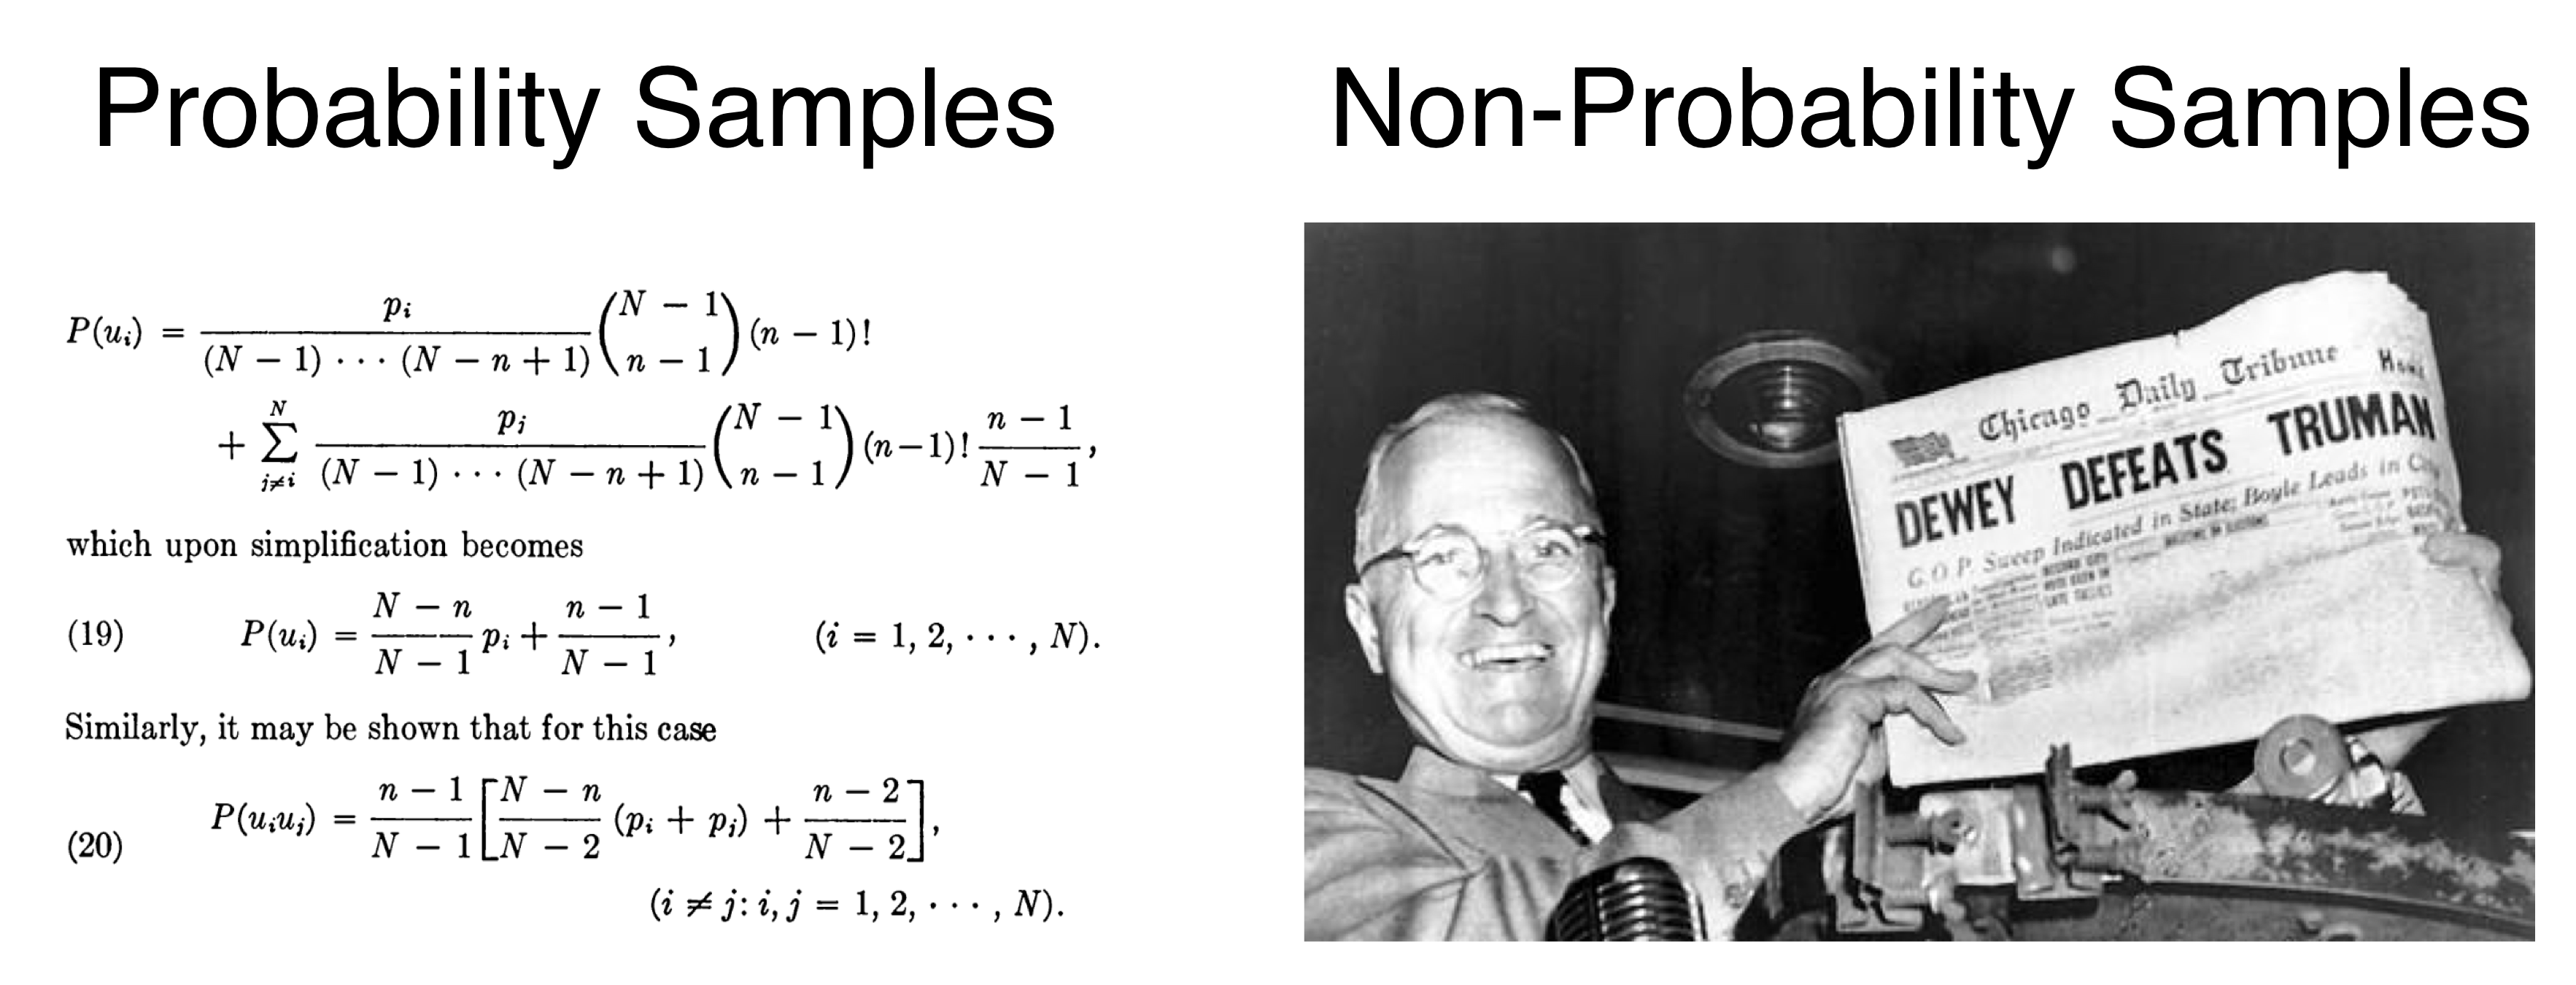
\includegraphics[width=\textwidth]{figures/prob_vs_nonprob_old}
\end{center}

\vf
\TINY{\url{http://www.chicagotribune.com/news/nationworld/politics/chi-chicagodays-deweydefeats-story-story.html}}

\end{frame}
%%%%%%%%%%%%%%%%%%%%%%%%%%%
\begin{frame}

\begin{center}
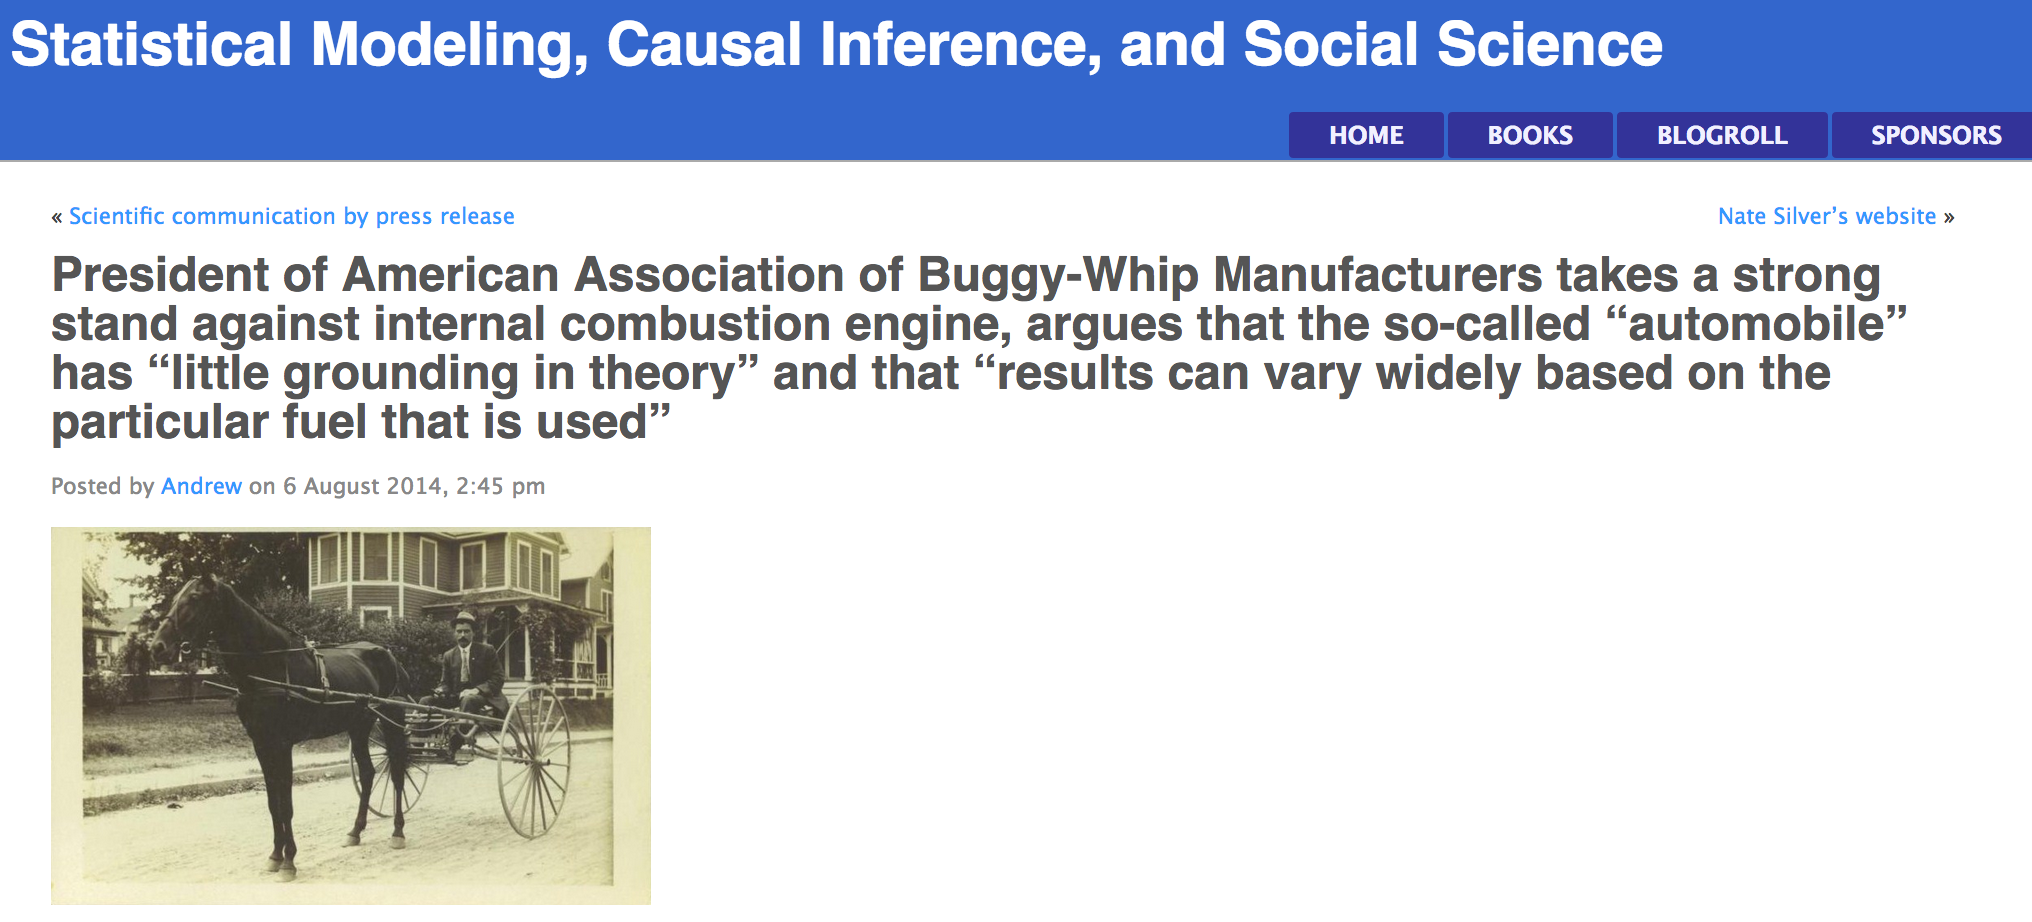
\includegraphics[width=0.9\textwidth]{figures/gelman_buggywhip_blogpost}
\end{center}

\vf
\TINY{\url{http://andrewgelman.com/2014/08/06/president-american-association-buggy-whip-manufacturers-takes-strong-stand-internal-combustion-engine-argues-called-automobile-little-grounding-theory/}}

\end{frame}
%%%%%%%%%%%%%%%%%%%%%%%%%%%
\begin{frame}

\begin{center}
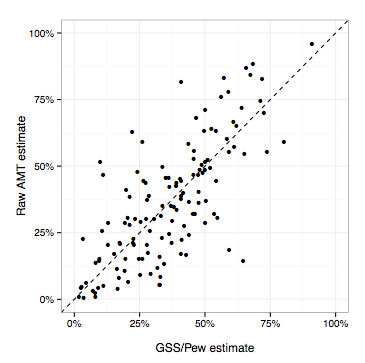
\includegraphics[width=0.5\textwidth]{figures/goel_non-representative_2016_fig1a}
\end{center}

\end{frame}
%%%%%%%%%%%%%%%%%%%%%%%%%%%
\begin{frame}

\begin{center}
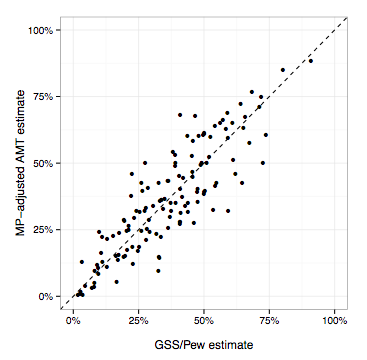
\includegraphics[width=0.5\textwidth]{figures/goel_non-representative_2016_fig2a}
\end{center}

\end{frame}
%%%%%%%%%%%%%%%%%%%%%%%%%%%
\begin{frame}

\begin{center}
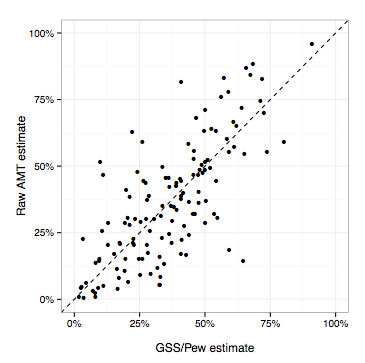
\includegraphics[width=0.4\textwidth]{figures/goel_non-representative_2016_fig1a}
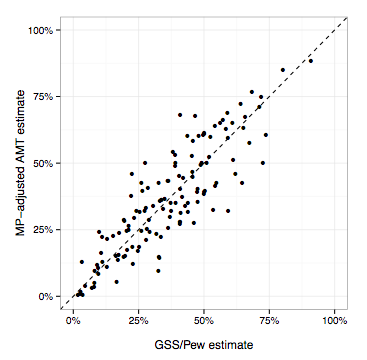
\includegraphics[width=0.4\textwidth]{figures/goel_non-representative_2016_fig2a}
\end{center}

\end{frame}
%%%%%%%%%%%%%%%%%%%%%%%%%%%
\begin{frame}

\begin{center}
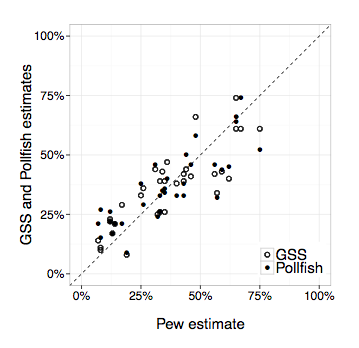
\includegraphics[width=0.5\textwidth]{figures/goel_non-representative_2016_fig4}
\end{center}

\end{frame}
%%%%%%%%%%%%%%%%%%%%%%%%%%%
\begin{frame}

\Large{
\begin{center}
What will happen if we try it again?
\end{center}
}

\end{frame}
%%%%%%%%%%%%%%%%%%%%%%%%%%%
\end{document}
